\documentclass[11pt,a4paper]{report}
\usepackage[utf8]{inputenc}
\usepackage[T1]{fontenc}
\usepackage{mathptmx}
\IfFileExists{french.ldf}{\usepackage[french]{babel}}{%
 \usepackage[english]{babel}%
 \AtBeginDocument{\renewcommand{\chaptername}{Chapitre}\renewcommand{\contentsname}{Table des matières}%
 \renewcommand{\figurename}{Figure}\renewcommand{\tablename}{Tableau}}}
\usepackage[margin=2.3cm]{geometry}
\usepackage{booktabs,longtable,tabularx,array,enumitem,xcolor,fancyhdr}
\usepackage{tikz}
\usetikzlibrary{arrows.meta,positioning}
\usepackage[colorlinks=true,linkcolor=blue!50!black,urlcolor=blue!50!black,citecolor=blue!50!black]{hyperref}

\setlength{\parskip}{4pt}
\setlength{\emergencystretch}{3em}
\setlength{\parindent}{0pt}
\setlist{itemsep=1pt,topsep=3pt}
\pagestyle{fancy}\fancyhf{}
\fancyhead[L]{\small Projet PAM --- Rapport technique}
\fancyhead[R]{\small TEK-UP 2026--2027}
\fancyfoot[C]{\thepage}
\renewcommand{\arraystretch}{1.15}

\newcommand{\aconf}{\emph{à confirmer}}
\newcommand{\amesurer}{\emph{à mesurer}}
\newcommand{\testfiche}[7]{%
\begin{center}\footnotesize
\begin{tabularx}{\textwidth}{@{}>{\bfseries}p{2.7cm}X@{}}
\toprule
\multicolumn{2}{@{}l}{\textbf{#1 --- #2}}\\ \midrule
Objectif & #3\\ Préconditions & #4\\ Procédure & #5\\
Résultat attendu & #6\\ Preuves à collecter & #7\\
Résultat observé & \amesurer{} (test non exécuté)\\ \bottomrule
\end{tabularx}\end{center}}

\begin{document}

%================= PAGE DE GARDE =================
\begin{titlepage}
\centering
\vspace*{1.5cm}
{\large TEK-UP --- Formation Cybersécurité\\Année universitaire 2026--2027\par}
\vspace{2cm}
{\Huge\bfseries Conception et mise en œuvre d'une solution de gestion des accès privilégiés (PAM)\par}
\vspace{1.2cm}
{
\begin{tabular}{rl}

 & \emph{Ayachi Yassine et Elheni Cyrine}\\
  & \emph{5-SSIR-A}\\

\end{tabular}}
\vfill
\end{titlepage}

\tableofcontents

%================= ACRONYMES =================
\chapter*{Liste des acronymes}
\addcontentsline{toc}{chapter}{Liste des acronymes}
\small
\begin{tabularx}{\textwidth}{@{}l X l X@{}}
AD DS & Active Directory Domain Services & MFA & Authentification multifacteur\\
BF / BNF & Besoin fonctionnel / non fonctionnel & MTTA & Mean Time to Acknowledge\\
DNS & Domain Name System & MTTD & Mean Time to Detect\\
CA & Autorité de certification & TOTP & Mot de passe à usage unique basé sur le temps\\
IAM & Gestion des identités et des accès & PAM & Gestion des accès privilégiés\\
IdP & Fournisseur d'identité & RBAC & Contrôle d'accès fondé sur les rôles\\
KPI & Indicateur de performance & SIEM & Gestion des événements de sécurité\\
LDAP & Lightweight Directory Access Protocol & SSO & Authentification unique\\
NTP & Network Time Protocol & XDR & Détection et réponse étendues\\
\end{tabularx}
\normalsize

%================= CHAPITRE 1 =================
\chapter{Introduction générale}

\section{Contexte et importance des comptes privilégiés}
Les infrastructures d'entreprise reposent sur des serveurs, des applications, des bases de données et des services interconnectés. Leur administration exige des privilèges élevés (comptes \texttt{root}, administrateurs de domaine, accès aux moteurs de conteneurs). Lorsque ces privilèges sont permanents, partagés, excessifs ou peu surveillés, la compromission d'un seul compte peut permettre de modifier des configurations, d'accéder à des données sensibles, d'installer des logiciels malveillants ou d'interrompre des services critiques.

Le risque est renforcé par la conteneurisation : selon la documentation de Docker, seuls des utilisateurs de confiance devraient pouvoir contrôler le démon Docker, qui requiert des privilèges \texttt{root} sauf en mode rootless~\cite{docker-sec}. L'accès au moteur Docker constitue donc lui-même un accès privilégié.

\section{Contexte et justification du projet}
Le projet consiste à construire un laboratoire représentatif d'une petite infrastructure d'entreprise pour étudier le contrôle des accès privilégiés, le moindre privilège, la traçabilité des opérations d'administration et la détection de comportements suspects. L'encadrant a précisé que l'architecture doit ressembler à un environnement d'entreprise et \textbf{inclure un pare-feu} ; les options de filtrage sont étudiées dans ce rapport, mais leur mise en œuvre reste à valider selon la topologie retenue.

\section{Problématique}
Comment centraliser et contrôler les accès privilégiés aux ressources d'une infrastructure, limiter l'administration non autorisée, assurer la traçabilité des opérations sensibles, et exploiter les événements de sécurité pour détecter et investiguer les tentatives de contournement, y compris les contournements par le réseau ?

\section{Objectif général et objectifs spécifiques}
\textbf{Objectif général.} Concevoir une architecture de laboratoire permettant d'étudier le contrôle des accès privilégiés à un serveur Linux et aux services qu'il héberge. Le déploiement et l'évaluation seront réalisés dans la mesure où les ressources, les licences et la topologie retenue le permettent.

\textbf{Objectifs spécifiques :}
\begin{itemize}
\item étudier les solutions IAM, PAM, SIEM et de filtrage réseau ;
\item déployer Active Directory (AD DS) et DNS comme référentiel d'identités ;
\item mettre en place une solution PAM (Teleport Community Edition envisagée) ;
\item héberger Nginx, une application Web/API et PostgreSQL dans des conteneurs Docker sur un serveur Linux ;
\item définir des rôles et appliquer le moindre privilège ;
\item restreindre les chemins d'accès directs contournant le PAM, par des règles de pare-feu notamment ;
\item collecter et analyser les journaux avec Wazuh ;
\item exécuter des tests d'autorisation, de refus, de traçabilité, de détection, de contournement et de filtrage ;
\item calculer les indicateurs uniquement pour les tests effectivement exécutés et documentés.
\end{itemize}

\section{Démarche méthodologique}
(1) étude de l'existant et des solutions à partir de la documentation officielle ; (2) analyse des besoins et des contraintes ; (3) conception préliminaire (architecture, flux, rôles, journalisation) ; (4) déploiement progressif ; (5) exécution des scénarios de test et collecte de preuves ; (6) calcul des indicateurs et rédaction des conclusions. \textbf{À la date de ce document, la phase 4 est partiellement réalisée et la phase 5 partiellement exécutée (chapitre~5) ; la phase 6 (indicateurs finaux) n'est pas réalisée.} Les affirmations sont classées en trois catégories : faits sourcés (avec référence), interprétations, décisions de conception.

\section{Périmètre et limites}
Le périmètre envisagé est un laboratoire local, sur un poste d'environ 16~Go de RAM. Le réseau Host-only, les composants retenus et leur emplacement restent à confirmer. Le cloud public, la haute disponibilité et le SSO Keycloak--Teleport CE ne sont pas prévus dans le périmètre initial (voir section~\ref{sec:perim}). Une fonction documentée par un éditeur ne sera considérée comme démontrée qu'après vérification ou test dans l'environnement retenu.

\section{Organisation du rapport}
Le chapitre~2 présente l'existant et compare les solutions ; le chapitre~3 formalise les besoins ; le chapitre~4 propose la conception préliminaire, dont la sous-section « Pare-feu et filtrage des flux réseau », la matrice des flux, l'analyse des menaces et le plan de tests ; le chapitre~5 présente la mise en œuvre réalisée et les résultats effectivement observés. La bibliographie et la liste des décisions ouvertes terminent le document.

%================= CHAPITRE 2 =================
\chapter{Étude de l'existant et étude comparative}

\section{État de l'existant}
\begin{itemize}
\item \textbf{Administration par SSH.} L'accès direct aux serveurs par SSH, souvent par clés statiques ou mots de passe, laisse peu de contrôle centralisé et une traçabilité limitée aux journaux locaux.
\item \textbf{Comptes privilégiés locaux et administrateurs.} Comptes partagés ou permanents : imputabilité faible, rotation rare, privilèges excédant le besoin.
\item \textbf{Annuaire.} Un annuaire (Active Directory) centralise utilisateurs et groupes, mais n'applique pas par lui-même le moindre privilège sur les serveurs Linux.
\item \textbf{Docker.} L'accès au démon équivaut à un accès privilégié sur l'hôte~\cite{docker-sec}. Par ailleurs, les ports publiés par Docker ne passent pas par les règles \texttt{INPUT} d'un pare-feu hôte comme \texttt{ufw} : Docker fournit la chaîne \texttt{DOCKER-USER} pour ce filtrage~\cite{docker-fw,baeldung-ufw}.
\item \textbf{Journalisation et supervision.} Journaux dispersés, non corrélés, rarement exploités sans SIEM.
\end{itemize}
\textbf{Limites} : privilèges permanents, contournements possibles (accès direct), journaux incomplets ou non centralisés, absence de filtrage réseau explicite entre les composants.

\section{Concepts et catégories de solutions}
\begin{longtable}{@{}p{2.6cm}p{13.2cm}@{}}
\toprule
\textbf{Notion} & \textbf{Définition retenue dans ce rapport}\\ \midrule\endhead
IAM & Gestion des identités et des droits associés (création, groupes, authentification, cycle de vie).\\
IdP & Service qui authentifie les utilisateurs et émet des assertions/jetons aux applications (ex. Keycloak).\\
PAM & Contrôle, limitation et audit des accès privilégiés aux ressources (serveurs, bases, conteneurs) : accès à la demande, durée limitée, enregistrement de sessions.\\
RBAC & Attribution des droits à des rôles, eux-mêmes attribués aux utilisateurs.\\
MFA & Authentification combinant au moins deux facteurs indépendants.\\
SIEM/XDR & Collecte, normalisation, corrélation et alerte sur les événements de sécurité.\\
Pare-feu & Filtrage des paquets selon des règles (adresse, port, sens). \textbf{Hôte} : sur chaque système ; \textbf{réseau/centralisé} : entre segments. Distinct de l'isolation fournie par le réseau virtuel.\\
Docker & Exécution d'applications dans des conteneurs partageant le noyau de l'hôte ; surface d'attaque propre au démon~\cite{docker-sec}.\\
Journalisation & Enregistrement horodaté des événements ; la corrélation et l'investigation exigent des horloges synchronisées et des sources complètes.\\
\bottomrule
\end{longtable}
\textbf{Principe directeur.} Ces catégories ne sont pas interchangeables : un IdP ne remplace pas un PAM, un SIEM ne remplace pas l'application des droits, et un pare-feu ne remplace pas le contrôle d'accès applicatif. Le choix final des outils dépendra des fonctions nécessaires, des contraintes de licence et des résultats de faisabilité.

\section{Étude comparative des solutions}
\subsection{Fiches synthétiques}
\textbf{Active Directory Domain Services (AD DS)} --- annuaire et authentification de domaine Windows. Points forts : standard d'entreprise, DNS intégré. Limites : ne contrôle pas les privilèges sur Linux/Docker ; l'utilisation des comptes AD dans Teleport n'est pas automatique (cahier des charges). Licence Windows Server à vérifier (évaluation).

\textbf{Keycloak} --- fournisseur d'identité (SSO, fédération LDAP/AD, MFA). Limite structurante : d'après la documentation de Teleport citée dans le cahier des charges~\cite{tp-keycloak}, l'intégration SSO Keycloak--Teleport nécessite Teleport Enterprise ; Teleport Community Edition ne prend en charge que GitHub comme fournisseur SSO externe. \textbf{Cette intégration n'est donc pas acquise} dans l'architecture retenue.

\textbf{Teleport Community Edition (candidate)} --- solution d'accès sécurisé à évaluer pour les ressources effectivement prises en charge. Les fonctions disponibles dépendent de la version et de l'édition. La documentation de licence indique des conditions d'éligibilité spécifiques depuis la version~16~\cite{tp-licence} ; la conformité de l'usage prévu doit être vérifiée avant de retenir cette solution.

\textbf{JumpServer} --- bastion/PAM open source (GPLv3) donnant accès à SSH, RDP, Kubernetes et bases via navigateur, avec audit de sessions~\cite{jumpserver}. Alternative crédible : interface Web native et intégration LDAP/AD annoncée ; empreinte probablement plus lourde (plusieurs composants), \amesurer{}.

\textbf{HashiCorp Boundary (Community)} --- accès par identité aux ressources. D'après une source indépendante~\cite{swi}, l'édition communautaire est sous licence BSL~1.1 (source-available) et l'enregistrement de sessions est réservé aux offres payantes ; à confirmer sur la documentation éditeur.

\textbf{Wazuh} --- plateforme de supervision : agents, manager, indexeur, tableau de bord~\cite{wazuh-arch}. Ne fait pas respecter les droits. Ports et transport dépendent de la version (voir section~\ref{sec:flux}).

\textbf{Docker Engine et Compose} --- exécution de conteneurs et description déclarative des services. Contraintes de sécurité : accès au démon, publication de ports et interaction avec le pare-feu~\cite{docker-sec,docker-fw}.

\subsection{Tableau comparatif}
\footnotesize
\begin{longtable}{@{}p{0.15\textwidth}p{0.24\textwidth}p{0.24\textwidth}p{0.24\textwidth}@{}}
\caption{Solutions d'accès privilégié (comparaison par critère)}\\
\toprule\textbf{Critère} & \textbf{Teleport CE} & \textbf{JumpServer} & \textbf{Boundary CE}\\ \midrule\endhead
Fonction principale & Accès sécurisé aux infrastructures & Bastion / PAM & Accès par identité\\
Contrôle des privilèges & Oui (rôles, accès contrôlé) & Oui (permissions d'assets) & Oui (à confirmer)\\
Gestion des identités & Locale (CE) ; SSO limité à GitHub & Locale ; LDAP/AD annoncé & Via IdP\\
Authentification / MFA & MFA selon configuration, à vérifier & MFA annoncé & Via IdP\\
Journalisation / audit & Audit, sessions prises en charge & Enregistrement et audit & Sessions : offres payantes~\cite{swi}\\
Lien avec AD & Pas automatique & LDAP/AD annoncé & À étudier\\
Linux et Docker & Cible Linux ; Docker non géré en interne & Cible Linux & Cible Linux\\
Facilité en laboratoire & Bonne & Moyenne (\amesurer) & Moyenne\\
Limites / licence & < 100 employés, < 10~M\$~\cite{tp-licence} & GPLv3 ; édition entreprise payante & BSL~1.1\\
\bottomrule
\end{longtable}

\begin{longtable}{@{}p{0.13\textwidth}p{0.18\textwidth}p{0.18\textwidth}p{0.18\textwidth}p{0.18\textwidth}@{}}
\caption{Identité, supervision et conteneurs (catégories distinctes, non interchangeables)}\\
\toprule\textbf{Critère} & \textbf{AD DS} & \textbf{Keycloak} & \textbf{Wazuh} & \textbf{Docker / Compose}\\ \midrule\endhead
Fonction principale & Annuaire, DNS & IdP / SSO & SIEM/XDR & Conteneurs\\
Contrôle des privilèges & Non (côté Linux) & Non & Non & Non\\
Gestion des identités & Oui & Oui & Non & Non\\
Authentification / MFA & Kerberos ; MFA selon configuration & MFA, SSO & Accès console & Non\\
Journalisation / audit & Journaux Windows & Événements d'authentification & Collecte, corrélation & Journaux Docker\\
Lien avec AD & Natif & Fédération possible & Collecte d'événements & ---\\
Linux et Docker & Hors périmètre & Application compatible & Agent Linux ; Docker à configurer & Natif\\
Facilité en laboratoire & Moyenne & Moyenne (ressources) & Déjà présent & Bonne\\
Limites / licence & Licence Windows & Intégration Teleport : Enterprise & Open source & Open source (versions à vérifier)\\
\bottomrule
\end{longtable}
\normalsize
\normalsize

\section{Justification du choix des composants}\label{sec:justif}
\begin{itemize}
\item \textbf{AD DS + DNS} : référentiel d'identités exigé par le cahier des charges (BF01). Rôle limité à l'annuaire et au DNS du domaine ; il n'est pas un fournisseur SSO de Teleport.
\item \textbf{Teleport Community Edition} : candidate à évaluer pour les accès Linux, les rôles et l'audit. La compatibilité avec les ressources, la licence applicable et les fonctions requises restent à vérifier avant décision.
\item \textbf{Wazuh} : présent en conteneurs sur le poste hôte ; la collecte des journaux du projet et les règles éventuelles restent à configurer et à tester.
\item \textbf{Docker Engine + Compose} : option envisagée pour héberger un service de test si la charge mémoire et la configuration le permettent.
\item \textbf{Keycloak} : conditionnel, pour la fédération AD ou une application compatible (BF13, T12) ; jamais présenté comme SSO de Teleport CE.
\item \textbf{JumpServer, Boundary} : étudiés comme alternatives, non retenus à ce stade ; JumpServer constitue le repli si Teleport CE se révèle inadapté (décision à valider).
\end{itemize}

\section{Synthèse de l'étude de l'existant}
\begin{longtable}{@{}p{5cm}p{10.8cm}@{}}
\toprule\textbf{Lacune identifiée} & \textbf{Réponse proposée}\\ \midrule\endhead
Accès SSH direct et privilèges permanents & PAM (Teleport) avec rôles ; blocage réseau du SSH direct\\
Identités non centralisées & AD DS/DNS ; Keycloak éventuel\\
Surface Docker & Droits Docker distincts (BF06), exposition minimale des ports, filtrage \texttt{DOCKER-USER}\\
Journaux dispersés & Wazuh, horloges synchronisées, journaux pare-feu\\
Réseau à plat sans filtrage & Pare-feu hôtes (recommandé), pare-feu centralisé en option\\
\bottomrule
\end{longtable}

%================= CHAPITRE 3 =================
\chapter{Analyse des besoins et cahier des charges}

\section{Problématique détaillée}
Un accès privilégié insuffisamment contrôlé expose à : l'escalade de privilèges, la modification non autorisée de configurations, l'accès aux données, la persistance d'un attaquant, et une impossibilité de reconstituer les faits. Deux contournements sont critiques : l'accès direct (SSH, base de données, API Docker) qui évite le PAM, et la supervision insuffisante qui empêche la détection.

\section{Objectifs mesurables}
Les cibles d'évaluation envisagées sont : vérifier les décisions RBAC sur la matrice définie ; tester le blocage des accès directs retenus ; vérifier la disponibilité des journaux et évaluer une règle de détection simple si les sources sont collectées ; contrôler les flux légitimes après filtrage. Les tests dépendant de composants non encore déployés seront reportés ou retirés du périmètre. Aucun taux de réussite n'est présumé ; les seuils seront confirmés avant les tests.

\section{Acteurs et rôles}
Profils logiques de test, associés ensuite aux mécanismes réellement configurés (rôles Teleport, groupes AD, comptes Linux, rôles PostgreSQL).
\begin{itemize}
\item \textbf{AI} Administrateur de l'infrastructure ; \textbf{OA} Opérateur applicatif ; \textbf{UL} Utilisateur à privilèges limités ;
\item \textbf{AS} Analyste sécurité ; \textbf{AP} Administrateur de la solution PAM.
\end{itemize}

\section{Besoins fonctionnels}
\footnotesize
\begin{longtable}{@{}p{1.2cm}p{5.2cm}p{1.8cm}p{1.4cm}p{4.6cm}@{}}
\toprule\textbf{ID} & \textbf{Description} & \textbf{Acteur} & \textbf{Priorité} & \textbf{Critère de validation}\\ \midrule\endhead
BF01 & Annuaire centralisé des identités et groupes du domaine de laboratoire & AP, AI & Haute & Domaine opérationnel, comptes de test créés, DNS résolu\\
BF02 & Autoriser/refuser l'accès aux ressources protégées selon les rôles PAM & AP, AI, OA, UL & Haute & Exactitude RBAC = 100~\% sur la matrice (T02, T03)\\
BF03 & Séparer au minimum administrateur, opérateur applicatif et utilisateur limité & AP & Haute & Matrice de permissions testée (T03, T04)\\
BF04 & Accès contrôlé aux ressources prises en charge par le PAM & AI, OA & Haute & T02\\
BF05 & Bloquer les connexions directes non autorisées vers le serveur cible & AI, AS & Haute & T01, T11, T13\\
BF06 & Réserver l'administration de Docker et de son socket aux acteurs autorisés & AI & Haute & T05\\
BF07 & Isoler les services (non-root, capacités limitées, ports minimaux, secrets protégés) & AI & Moyenne & Revue du fichier Compose ; T09\\
BF08 & Journaliser utilisateur, heure, ressource, origine, résultat quand disponibles & AS & Haute & Couverture de journalisation (T08, T10)\\
BF09 & Centraliser les événements pertinents dans Wazuh & AS & Haute & Événements visibles dans Wazuh\\
BF10 & Règles pour échecs répétés, accès interdit, modification sensible, activité inhabituelle & AS & Haute & T07 ; taux de détection, MTTD\\
BF11 & Reconstituer une chronologie à partir des journaux & AS & Moyenne & T08, T10\\
BF12 & Mesurer l'efficacité par scénarios et indicateurs & AI, AS & Haute & Indicateurs calculés sur résultats réels\\
BF13 & Évaluer Keycloak et la fédération AD (optionnel) & AP & Basse & T12, si retenu et supporté\\
BF14  & Filtrer le trafic par pare-feu hôtes et, si retenu, filtrage centralisé & AI & Haute & Règles documentées et actives ; T13--T16\\
BF15  & N'autoriser que les communications nécessaires aux services et chemins d'administration & AI & Haute & Matrice des flux conforme aux règles ; T16, T18\\
BF16  & Empêcher les connexions directes non autorisées, dont le SSH direct du scénario de contournement & AI, AS & Haute & T13 (et T01, T11)\\
BF17  & Collecter les événements de pare-feu si la configuration le permet, et les intégrer à la supervision & AS & Moyenne & T17\\
\bottomrule
\end{longtable}
\normalsize

\section{Besoins non fonctionnels}
\footnotesize
\begin{longtable}{@{}p{1.4cm}p{7.6cm}p{6.2cm}@{}}
\toprule\textbf{ID} & \textbf{Description} & \textbf{Critère de validation}\\ \midrule\endhead
BNF01 & Sécurité : moindre privilège, interfaces d'administration limitées, secrets protégés & Revue de configuration ; aucun secret dans le dépôt\\
BNF02 & Isolation : réseau de laboratoire isolé, communications limitées au nécessaire & Réseau Host-only~\cite{vmware-ho} + règles (T16)\\
BNF03 & Traçabilité : horloges synchronisées, journaux horodatés & Écart d'horloge mesuré avant les tests\\
BNF04 & Performance : fonctionnement sur environ 16~Go de RAM & Toutes les VM actives sans saturation mémoire (\amesurer)\\
BNF05 & Maintenabilité : configurations documentées, reproductibles, versionnées & Dépôt de configurations expurgées\\
BNF06 & Disponibilité du laboratoire : redémarrage indépendant, restauration par snapshots & Snapshot et restauration testés\\
BNF07 & Évolutivité : ajout de rôles, services, scénarios & Ajout d'un rôle de test sans refonte\\
BNF08 & Auditabilité : tests, résultats et limites documentés & Fiches de test complétées\\
BNF09 & Compatibilité : versions et fonctions vérifiées avant chaque intégration & Tableau des versions\\
BNF10 & Confidentialité : comptes et données de test uniquement & Revue des jeux de données\\
BNF11  & Défense en profondeur : isolation, filtrage, contrôle d'accès, journalisation & Chaque couche testée séparément\\
BNF12  & Minimisation de la surface d'attaque : aucun port ou service superflu exposé & T16\\
BNF13  & Maintenabilité des règles : règles de pare-feu documentées et justifiées & Chaque règle liée à une ligne de la matrice des flux\\
BNF14  & Compatibilité avec les ressources : aucune VM supplémentaire dédiée au pare-feu & Inventaire des VM inchangé\\
\bottomrule
\end{longtable}
\normalsize

\section{Contraintes}
Ressources limitées (environ 16~Go) ; fonctions dépendantes de l'édition (Teleport CE, licence~\cite{tp-licence}) ; limites d'intégration (pas de SSO Keycloak--Teleport CE) ; risque d'escalade par Docker ; disponibilité et qualité des journaux ; réseau isolé nécessaire ; dépendances et versions (Wazuh : ports différents selon les versions~\cite{wazuh-arch}) ; rôle final d'Ubuntu Server non fixé ; disponibilité de Kali à confirmer.

\section{Périmètre et hors périmètre}\label{sec:perim}
\begin{tabularx}{\textwidth}{@{}XX@{}}
\toprule\textbf{Périmètre envisagé (à valider)} & \textbf{À valider / hors périmètre}\\ \midrule
AD DS/DNS ; évaluation PAM ; un service Linux de test ; Wazuh si collecte possible ; pare-feu hôtes ; scénarios sélectionnés parmi T01--T18 & Keycloak (conditionnel) ; pare-feu centralisé sur Ubuntu (option A) ; JumpServer (repli) ; cloud public ; haute disponibilité ; SSO Keycloak--Teleport CE ; licence commerciale ; SOAR ; contrôle de chaque action métier dans les conteneurs\\
\bottomrule
\end{tabularx}

\section{Critères d'acceptation}
Les critères d'acceptation définitifs seront ajustés au périmètre validé avec l'encadrant. À minima, le rapport final devra distinguer les composants installés des composants seulement envisagés, documenter les règles et tests réellement réalisés, présenter les preuves disponibles, calculer les indicateurs uniquement lorsque les données existent et exposer les limites rencontrées. Les scénarios dépendant d'un composant non retenu ne seront pas présentés comme réussis.

%================= CHAPITRE 4 =================
\chapter{Conception préliminaire de la solution}

\section{État de l'environnement et hypothèses de déploiement}
\textit{Cette section décrit l'état au moment de la conception. L'environnement effectivement construit (trois VM Linux/Windows, Teleport, Docker, pare-feu) est décrit au chapitre~\ref{chap:real}.}

À la date de rédaction, les seules machines de laboratoire confirmées pour ce projet sont une VM Windows Server destinée à AD DS/DNS et une VM Ubuntu Server. Wazuh est déjà exécuté en conteneurs Docker sur le poste hôte Windows. La disponibilité et la topologie définitive de Kali Linux pour les tests doivent être confirmées dans l'inventaire final. Aucun serveur Teleport séparé, serveur applicatif séparé ni pare-feu dédié n'est considéré comme déjà installé.

La suite du rapport distingue donc l'architecture logique cible des machines effectivement disponibles. Les rôles logiciels ne correspondent pas automatiquement à des VM distinctes. Le rôle final d'Ubuntu Server et l'emplacement d'exécution de Teleport restent à décider. Pour préserver la valeur du contrôle PAM, Teleport et la ressource protégée ne devraient pas partager la même frontière d'administration si cela peut être évité ; si la contrainte de ressources impose une colocalisation temporaire, cette limite devra être explicitement documentée et les résultats ne devront pas être présentés comme équivalents à une séparation en production.

Aucune VM supplémentaire ne sera créée uniquement pour le pare-feu. Le filtrage de base repose sur les pare-feu natifs des systèmes. Un pare-feu/routeur centralisé réutilisant Ubuntu ne sera envisagé qu'après validation d'une topologie à plusieurs réseaux et d'un rôle exclusif pour Ubuntu.

\section{Architecture logique}
La figure suivante représente les fonctions visées, et non un inventaire de VM déjà déployées. Les deux machines confirmées sont Windows Server (AD DS/DNS) et Ubuntu Server ; Wazuh est actuellement hébergé en conteneurs sur le poste Windows hôte. Les composants Teleport, Docker et les services applicatifs sont des rôles cibles dont l'affectation physique reste à valider.

\begin{figure}[htbp]
\centering
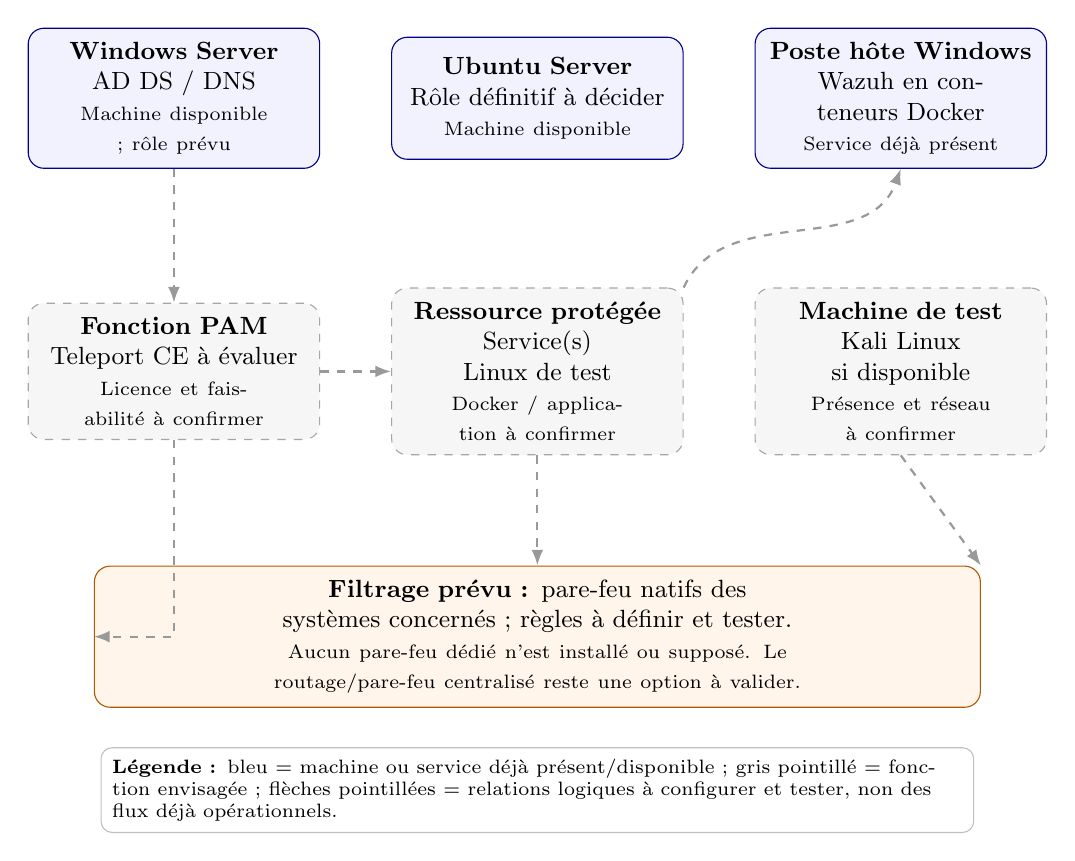
\begin{tikzpicture}[
  font=\small,
  node distance=8mm and 9mm,
  confirmed/.style={draw=blue!55!black,fill=blue!5,rounded corners=2mm,
    align=center,text width=3.35cm,minimum height=1.55cm,inner sep=5pt},
  planned/.style={draw=gray!70,fill=gray!7,rounded corners=2mm,dashed,
    align=center,text width=3.35cm,minimum height=1.55cm,inner sep=5pt},
  filter/.style={draw=orange!70!black,fill=orange!8,rounded corners=2mm,
    align=center,text width=10.9cm,minimum height=1.0cm,inner sep=5pt},
  link/.style={-{Latex[length=2mm]},thick},
  possible/.style={-{Latex[length=2mm]},thick,dashed,gray!80},
  lab/.style={font=\scriptsize,align=center,text width=3.2cm}
]
% Confirmed inventory: top row
\node[confirmed] (dc) {\textbf{Windows Server}\par AD DS / DNS\par\scriptsize Machine disponible ; rôle prévu};
\node[confirmed,right=of dc] (ubuntu) {\textbf{Ubuntu Server}\par Rôle définitif à décider\par\scriptsize Machine disponible};
\node[confirmed,right=of ubuntu] (host) {\textbf{Poste hôte Windows}\par Wazuh en conteneurs Docker\par\scriptsize Service déjà présent};

% Logical functions: second row, explicitly planned
\node[planned,below=17mm of dc] (pam) {\textbf{Fonction PAM}\par Teleport CE à évaluer\par\scriptsize Licence et faisabilité à confirmer};
\node[planned,right=of pam] (target) {\textbf{Ressource protégée}\par Service(s) Linux de test\par\scriptsize Docker / application à confirmer};
\node[planned,right=of target] (test) {\textbf{Machine de test}\par Kali Linux si disponible\par\scriptsize Présence et réseau à confirmer};

% Filter layer applies to hosts; it is not shown as a separate appliance.
\node[filter,below=14mm of target] (fw) {\textbf{Filtrage prévu :} pare-feu natifs des systèmes concernés ; règles à définir et tester.\\
\scriptsize Aucun pare-feu dédié n'est installé ou supposé. Le routage/pare-feu centralisé reste une option à valider.};

% Only logical relations; no arrow implies a configured flow.
\draw[possible] (dc.south) -- (pam.north);
\draw[possible] (pam.east) -- (target.west);
\draw[possible] (target.north east) to[out=65,in=250] (host.south);
\draw[possible] (test.south) -- (fw.north east);
\draw[possible] (pam.south) |- (fw.west);
\draw[possible] (target.south) -- (fw.north);

\node[draw=gray!50,rounded corners,inner sep=4pt,align=left,font=\scriptsize,
  below=5mm of fw,text width=10.8cm] (legend)
  {\textbf{Légende :} bleu = machine ou service déjà présent/disponible ; gris pointillé = fonction envisagée ; flèches pointillées = relations logiques à configurer et tester, non des flux déjà opérationnels.};
\end{tikzpicture}
\caption{Architecture logique cible et distinction entre inventaire disponible et fonctions envisagées}
\label{fig:architecture-logique}
\end{figure}

\textbf{Rôles.} AD DS/DNS fournit l'annuaire et la résolution de noms du domaine de laboratoire. Teleport est la passerelle logique d'accès privilégié aux ressources qu'il prend en charge, mais son emplacement n'est pas encore fixé. Ubuntu Server est disponible, mais sa fonction (cible applicative, service PAM ou routeur/pare-feu) doit être décidée avant l'installation. Wazuh pourra servir à la collecte et à l'analyse des événements retenus ; sa présence sur le poste hôte ne signifie pas que les journaux du laboratoire y sont déjà envoyés. Le filtrage est assuré d'abord par les pare-feu des hôtes. Keycloak demeure optionnel et ne fait pas partie du chemin SSO de Teleport Community Edition.

\section{Plan d'adressage}
\textit{Mise à jour : le réseau VMnet1 et les adresses 192.168.70.10 (DC-01), .20 (GW01), .30 (TARGET01) et .1 (PC) sont désormais affectés et vérifiés (chapitre~\ref{chap:real}) ; le texte suivant correspond à la phase de conception.} Le réseau VMware Host-only et les adresses IP n'étaient pas encore confirmés à cette phase. Le sous-réseau \texttt{192.168.70.0/24} est une hypothèse de travail uniquement ; il ne devra être utilisé qu'après vérification de l'absence de conflit avec le réseau local et les réseaux virtuels existants. Les adresses du contrôleur de domaine, d'Ubuntu, du poste hôte et de la machine de test seront attribuées après validation de la topologie ; les suffixes \texttt{.10}, \texttt{.20}, \texttt{.30} et \texttt{.40} présents dans certains scénarios initiaux ne sont pas des adresses actuellement affectées. Le réseau Host-only fournit une isolation vis-à-vis du réseau physique, mais ne filtre pas à lui seul les flux entre machines virtuelles~\cite{vmware-ho}.

\section{Pare-feu et filtrage des flux réseau}\label{sec:pf}
\subsection{Rôle dans la défense en profondeur}
Le pare-feu contrôle l'\emph{accessibilité réseau} ; le PAM contrôle l'\emph{accès privilégié} aux ressources qu'il prend en charge. Aucun ne remplace l'autre : un SSH direct autorisé par le réseau contourne le PAM, et un PAM sans filtrage peut être contourné par le chemin réseau. La couche de filtrage complète l'isolation, le contrôle d'accès et la journalisation (BNF11).

\subsection{Isolation, pare-feu hôte et pare-feu centralisé}
\begin{tabularx}{\textwidth}{@{}p{2.8cm}XXX@{}}
\toprule & \textbf{Host-only (VMware)} & \textbf{Pare-feu hôte} & \textbf{Pare-feu centralisé}\\ \midrule
Rôle & Isole le laboratoire du réseau physique~\cite{vmware-ho} & Filtre le trafic entrant/sortant d'un système & Filtre le trafic entre segments\\
Granularité & Réseau entier & Par machine, par port, par source & Par segment ou par flux\\
Limite & Pas de politique de flux entre VM d'un même réseau & Gérée sur chaque machine ; modifiable par un administrateur local compromis & Point unique à protéger ; exige routage et interfaces multiples\\
\bottomrule
\end{tabularx}

Le Host-only n'est donc \textbf{pas} un pare-feu d'entreprise : il isole, il ne filtre pas les flux entre VM.

\subsection{Étude des options}\label{sec:optab}
\textbf{Option A --- Réutiliser Ubuntu Server comme pare-feu/routeur.} Ubuntu utilise Netfilter ; \texttt{nftables} est le moteur moderne et \texttt{ufw} un frontal simplifié~\cite{ubuntu-fw}. Prérequis : deux interfaces au moins sur deux réseaux Host-only distincts (le Virtual Network Editor permet plusieurs réseaux Host-only~\cite{vmware-multi}), activation du routage IPv4, routes ou passerelle sur chaque VM, et un rôle exclusif. \textbf{Non faisable tant que le rôle final et la topologie d'Ubuntu ne sont pas fixés.} Si Ubuntu est aussi la cible Docker, une machine compromise contrôlerait le filtre : combinaison déconseillée ; si Ubuntu est aussi le serveur Teleport, le point d'entrée et le routeur partagent le même risque : compromis à documenter.

\textbf{Option B --- Pare-feu natifs.} Windows Defender Firewall sur Windows Server et \texttt{ufw}/\texttt{nftables} sur les machines Linux, avec Host-only pour l'isolation. Point d'attention : les ports publiés par Docker contournent les règles \texttt{INPUT} d'\texttt{ufw} ; il faut ne pas publier les ports inutiles, ou filtrer dans \texttt{DOCKER-USER}~\cite{docker-fw,baeldung-ufw}.

\begin{tabularx}{\textwidth}{@{}p{2.6cm}XX@{}}
\toprule\textbf{Critère} & \textbf{A : Ubuntu routeur} & \textbf{B : pare-feu natifs}\\ \midrule
Sécurité & Point de contrôle entre segments ; point unique de défaillance & Filtrage par hôte ; réseau plat, pas de filtrage entre segments\\
Complexité & Élevée (2 interfaces, routage, routes) & Modérée (deux familles d'outils)\\
Ressources & Pas de VM ajoutée, mais Ubuntu mobilisé & Négligeables\\
Testabilité & Tests inter-segments clairs, journaux centralisés & Tests par hôte, journaux hétérogènes\\
Adéquation & Plus proche d'une architecture d'entreprise ; dépend du rôle d'Ubuntu & Faisable avec l'existant dès maintenant\\
\bottomrule
\end{tabularx}

\textbf{Option de départ proposée.} Utiliser les pare-feu natifs comme mesure de base, sans ajouter de VM, sous réserve de l'accord de l'encadrant. Cette option permet de filtrer les accès à chaque système et de documenter les règles, mais elle ne constitue pas un pare-feu réseau centralisé entre segments. Comme l'encadrant a demandé un pare-feu dans l'architecture d'entreprise, il faut lui faire valider explicitement si le filtrage hôte répond à cette exigence. Si un équipement centralisé est obligatoire, l'option A devra être étudiée après attribution d'un rôle exclusif à Ubuntu et mise en place de deux réseaux distincts ; elle ne doit pas être représentée comme déployée à ce stade.

\subsection{Segmentation, moindre privilège et anti-contournement}
\begin{itemize}
\item \textbf{Zones logiques} : identité (DC), accès (PAM), charge de travail (TARGET), supervision (Wazuh), test (Kali). Appliquées par règles d'hôtes (option B) ou par segments physiques (option A).
\item \textbf{Moindre privilège réseau} : politique par défaut « refuser » en entrée ; ouvertures nominatives par source, destination et port ; sortie restreinte aux destinations nécessaires. Les ports Teleport, Wazuh et AD sont à confirmer selon les versions, les rôles réellement installés et la configuration retenue ; les valeurs indicatives de la matrice ne sont pas des règles à appliquer sans vérification.
\item \textbf{Contournement SSH} : le SSH direct vers serveur cible Linux est refusé aux sources non autorisées ; la connexion Teleport--cible reste fonctionnelle. Selon la variante, la cible n'ouvre que le port d'écoute Teleport depuis l'adresse du serveur PAM (connexion directe, port \texttt{3022} par défaut), ou n'ouvre aucun port entrant de gestion (l'agent établit un tunnel inverse sortant vers le Proxy)~\cite{tp-net}. Un accès de secours (console de la VM) est à prévoir et documenter.
\item \textbf{Docker et PostgreSQL} : API Docker jamais exposée en TCP ; PostgreSQL non publié sur l'hôte et joint seulement via un réseau Docker interne dédié ; Nginx seul point d'entrée applicatif.
\item \textbf{Journalisation} : \texttt{ufw} peut activer la journalisation~\cite{ufw-wiki} ; \texttt{nftables} via la cible \texttt{log} avec préfixe ; journal des paquets rejetés de Windows Defender Firewall à activer (à vérifier). L'ingestion par Wazuh et le décodage sont \textbf{à valider} ; le volume de journaux doit être limité aux refus et aux flux de test.
\end{itemize}

\textbf{Limites.} Un pare-feu ne prévient pas l'escalade de privilèges d'un utilisateur déjà doté de permissions locales excessives et ne remplace pas les contrôles d'autorisation des applications ou de PostgreSQL.

\section{Matrice des flux réseau (proposée)}\label{sec:flux}
{\setlength{\tabcolsep}{3pt}\scriptsize
\begin{longtable}{@{}p{0.12\textwidth}p{0.11\textwidth}p{0.22\textwidth}p{0.12\textwidth}p{0.24\textwidth}p{0.09\textwidth}@{}}
\caption{Matrice indicative des flux --- hypothèses à confirmer avant toute configuration}\\
\toprule\textbf{Source} & \textbf{Destination} & \textbf{Protocole/port} & \textbf{Objet} & \textbf{Politique proposée} & \textbf{Validation}\\ \midrule\endhead
Poste d'admin autorisé (à désigner) & Service Teleport (emplacement à confirmer) & TCP 443 (routage TLS) ou 3080~\cite{tp-net} ; \aconf{} & Point d'entrée Teleport & Autoriser depuis les sources d'admin désignées seulement & T02, T18\\
Service Teleport & serveur cible Linux (emplacement à confirmer) & Variante tunnel inverse : sortant de la cible vers le Proxy (443 ou 3024) ; variante connexion directe : TCP 3022 vers la cible~\cite{tp-net} ; \aconf{} selon la configuration retenue & Accès SSH géré par le PAM & Autoriser uniquement la variante retenue, avec l'adresse du serveur PAM comme seule source & T02, T13, T18\\
machine de test autorisée (Kali, disponibilité à confirmer) & serveur cible Linux (emplacement à confirmer) & TCP 22 & Tentative de contournement du PAM & Refuser et journaliser (DROP ou REJECT : décision à valider) & T01, T11, T13\\
Conteneur application & Conteneur PostgreSQL & TCP 5432, réseau Docker interne & Accès base par l'application & Autoriser sur le réseau Docker interne dédié ; 5432 non publié sur l'hôte & T09, T14\\
Source non autorisée (Kali) & serveur cible Linux & TCP 5432 & Accès direct à PostgreSQL & Refuser (port non publié + règle hôte) & T14, T16\\
Membres du domaine / composants & Windows Server (AD DS/DNS) & DNS 53, Kerberos 88, LDAP 389 et autres ports AD ; \aconf{} (documentation Microsoft à vérifier) & Résolution DNS, authentification, jointure & Autoriser depuis les membres du domaine uniquement & T18\\
Hôte cible Linux (agent Wazuh si installé) & Manager Wazuh & TCP 1514 (événements) et 1515 (enrôlement) pour les agents 4.x ; 1517/TCP pour les agents 5.x~\cite{wazuh-arch,wazuh-enrol} ; \aconf{} selon la version & Remontée des événements & Autoriser en sortie vers l'adresse du manager seulement & T17, T18\\
Hôte exécutant Teleport (agent Wazuh si installé) & Manager Wazuh & Mêmes ports, \aconf{} & Journaux d'audit Teleport & Idem & T10, T18\\
Clients autorisés & Nginx (TARGET) & TCP 80/443 selon la configuration & Accès à l'application & Autoriser depuis les clients autorisés & T15\\
Toute source & TARGET : API Docker & TCP 2375/2376 & Administration Docker & Refuser ; socket Unix local uniquement & T05, T16\\
Toute source & TARGET : autres ports entrants & Tous, hors ports ouverts ci-dessus & Réduction de surface & Refuser par défaut & T16\\
Machines du laboratoire & Internet / autres réseaux & Tous & Contrôle du sortant & Refuser par défaut ; Host-only n'offre pas d'accès Internet par défaut~\cite{vmware-ho-doc} ; exceptions temporaires documentées & T16, T18\\
\bottomrule
\end{longtable}}
\normalsize

\section{Matrice initiale des rôles et permissions (proposée)}
\begin{tabularx}{\textwidth}{@{}p{3.6cm}XXXXX@{}}
\toprule\textbf{Ressource} & \textbf{AI} & \textbf{OA} & \textbf{UL} & \textbf{AS} & \textbf{AP}\\ \midrule
Accès à la ressource cible via Teleport & Oui & Oui (compte limité) & Non & Non & Non\\
Élévation d'administration système & Oui & Non & Non & Non & Non\\
Administration Docker & Oui & Limité (à définir) & Non & Non & Non\\
Configuration Nginx protégée & Écriture & Rechargement (à définir) & Non & Non & Non\\
Administration PostgreSQL & Oui & Non (compte applicatif) & Non & Non & Non\\
Utilisation de l'application & Oui & Oui & Oui & --- & ---\\
Console Wazuh & Lecture & Non & Non & Oui & Non\\
Administration de Teleport & Non & Non & Non & Non & Oui\\
\bottomrule
\end{tabularx}
\textit{Le périmètre « Limité » de l'opérateur applicatif sur Docker est un point de risque : toute commande permettant de piloter Docker peut donner un accès équivalent à \texttt{root}~\cite{docker-sec}. Son mécanisme est à définir.}

\section{Analyse des menaces liées au filtrage}
\footnotesize
\begin{longtable}{@{}p{2.9cm}p{5.5cm}p{6.2cm}@{}}
\toprule\textbf{Menace} & \textbf{Mesure proposée} & \textbf{Preuve d'efficacité}\\ \midrule\endhead
Accès réseau non autorisé & Politique par défaut « refuser », ouvertures nominatives & Scan depuis Kali : ports fermés (T16)\\
SSH direct contournant le PAM & Refus du SSH direct hors chemin Teleport & Échec du SSH direct, succès via Teleport (T13)\\
Accès non autorisé à PostgreSQL & Port non publié, réseau Docker interne, règle hôte & Connexion refusée depuis Kali, application fonctionnelle (T14)\\
Exposition de l'administration Docker & Pas d'API TCP ; socket local ; droits Docker restreints & Port 2375/2376 fermé ; accès refusé (T05, T16)\\
Blocage accidentel de services légitimes & Règles testées et fiches de non-régression & AD/DNS, Teleport et Wazuh fonctionnels (T18)\\
Règles mal configurées (dont contournement Docker du pare-feu) & Revue de règles, \texttt{DOCKER-USER}~\cite{docker-fw}, snapshot avant modification & Comparaison matrice des flux et règles actives\\
Journaux de pare-feu absents ou incomplets & Activation de la journalisation, test d'ingestion & Événement généré visible dans Wazuh, ou limite documentée (T17)\\
\bottomrule
\end{longtable}
\normalsize

\section{Stratégie de collecte des journaux}
Sources : système Linux (agent Wazuh sur l'hôte), authentification, audit Teleport, événements Docker configurés, Nginx et applicatifs, événements AD pertinents, journaux de pare-feu. Les règles de détection sont élaborées à partir des journaux réellement collectés et ne sont validées qu'après test. Les horloges sont synchronisées (source de temps unique, à définir) avant toute mesure.

\section{Plan de tests}
Les tests ci-dessous constituent un catalogue de scénarios candidats, pas un engagement à les exécuter tous. Les scénarios retenus seront adaptés à la topologie approuvée et aux composants effectivement installés. Avant chaque test, vérifier l'autorisation, les comptes de test, la possibilité de restauration et les préconditions propres au scénario. Les résultats observés sont à renseigner après exécution ; une précondition absente entraîne le report ou le retrait du test, et non une réussite présumée.

\subsection{Tests T01 à T12 (synthèse)}
\footnotesize
\begin{longtable}{@{}p{0.9cm}p{4.2cm}p{4.2cm}p{3.2cm}p{1.6cm}@{}}
\toprule\textbf{ID} & \textbf{Scénario} & \textbf{Résultat attendu} & \textbf{Preuves} & \textbf{Observé}\\ \midrule\endhead
T01 & SSH direct non autorisé & Refus, événement exploitable & Sortie client, journaux & \amesurer\\
T02 & Accès via le chemin PAM autorisé & Connexion réussie selon le rôle & Audit Teleport & Réussi (A2, ch.~5)\\
T03 & Action privilégiée par utilisateur sans rôle & Refus & Journaux sudo/Teleport & Réussi (A5, ch.~5)\\
T04 & Opérateur gère un service autorisé & Action permise dans le périmètre & Journaux & \amesurer\\
T05 & Administration Docker non autorisée & Refus & Journaux Docker/système & Réussi (A6, ch.~5)\\
T06 & Modification non autorisée de la configuration Nginx & Blocage et/ou événement détectable & Journaux, alerte & \amesurer\\
T07 & Échecs d'authentification répétés & Événements collectés, détection évaluée & Alertes Wazuh, horodatages & \amesurer\\
T08 & Activité administrative autorisée & Journaux exploitables pour l'investigation & Chronologie & \amesurer\\
T09 & Action sensible PostgreSQL via compte applicatif & Refus selon privilèges & Journaux PostgreSQL & \amesurer\\
T10 & Corrélation PAM, système, applicatif & Chronologie reconstituable si données disponibles & Export corrélé & \amesurer\\
T11 & Contournement du chemin PAM & Bloqué, ou faiblesse identifiée et corrigée & Rapport de test & \amesurer\\
T12 & Keycloak (si retenu et supporté) & Évaluation de la fédération AD & Notes de test & \amesurer\\
\bottomrule
\end{longtable}
\normalsize

\subsection{Tests de pare-feu T13 à T18}
\textit{Les fiches ci-dessous restent le protocole prévu. Les tests F1 à F9 du chapitre~\ref{chap:real} en constituent une exécution partielle, depuis GW01 et le PC et non depuis Kali ; aucune fiche n'est donc considérée comme réussie à ce stade.}

\testfiche{T13}{SSH direct non autorisé}{Vérifier que le SSH direct interdit est bloqué et que l'accès Teleport autorisé reste fonctionnel}{Règles hôte actives sur la cible retenue ; Teleport opérationnel et son emplacement confirmé ; compte de test valide ; source Kali hors liste d'autorisation}{1) Depuis Kali, tenter un SSH vers \texttt{<adresse\_IP\_cible>:22}. 2) Depuis le poste autorisé, se connecter via Teleport. 3) Relever les journaux}{1) refus ou délai dépassé, avec événement de pare-feu ; 2) connexion réussie}{Sorties de commande, journaux de pare-feu et Teleport, horodatages}

\testfiche{T14}{Isolation de PostgreSQL}{Vérifier que PostgreSQL n'est joignable que par l'application}{Si les services Docker sont retenus : port 5432 non publié ; réseau Docker interne dédié}{1) Depuis Kali, test de connexion vers \texttt{<adresse\_IP\_cible>:5432}. 2) Depuis l'application, requête de test légitime}{1) échec de connexion ; 2) requête réussie}{Sorties de test, journaux applicatifs, configuration Compose expurgée}

\testfiche{T15}{Exposition du service Web}{Vérifier que seuls les clients prévus atteignent Nginx}{Nginx exposé sur les ports retenus ; liste des clients autorisés définie}{1) Accès depuis un client autorisé. 2) Accès depuis un client non autorisé}{1) réponse HTTP ; 2) refus ou absence de réponse}{Réponses HTTP, journaux Nginx et pare-feu}

\testfiche{T16}{Ports entrants inutiles}{Vérifier que les ports non nécessaires sont fermés ou filtrés}{Matrice des flux figée ; règles appliquées}{Scan de ports des hôtes effectivement déployés depuis la machine de test autorisée ; comparaison avec la matrice}{Seuls les ports de la matrice répondent}{Résultats du scan, règles actives exportées}

\testfiche{T17}{Journalisation du pare-feu}{Vérifier qu'un refus ou une autorisation contrôlée est journalisé et visible dans Wazuh}{Journalisation activée ; collecte Wazuh configurée (à valider)}{Générer une connexion refusée contrôlée ; chercher l'événement localement puis dans Wazuh}{Événement présent localement ; présent dans Wazuh si configuré}{Extrait de journal, alerte ou événement Wazuh, horodatages}

\testfiche{T18}{Régression du trafic légitime}{Vérifier que les règles ne bloquent pas AD/DNS, Teleport ni Wazuh}{Topologie et composants retenus démarrés ; règles de pare-feu appliquées}{Résolution DNS ; authentification de domaine ; connexion Teleport ; remontée d'événements Wazuh}{Tous les flux essentiels fonctionnent}{Sorties de test, journaux de chaque composant}

\section{Indicateurs prévus}
Formules et méthode uniquement ; aucune valeur n'est établie.
\begin{itemize}
\item Exactitude RBAC = décisions conformes à la matrice / total des tests d'autorisation $\times$ 100.
\item Taux de blocage = tentatives non autorisées bloquées / tentatives non autorisées testées $\times$ 100.
\item Couverture de journalisation = événements attendus journalisés / événements attendus testés $\times$ 100.
\item Taux de détection = événements détectés / événements détectables $\times$ 100.
\item MTTD = horodatage de détection $-$ horodatage de l'événement ; MTTA = horodatage de prise en charge $-$ horodatage de détection.
\item Préservation des flux légitimes = flux essentiels fonctionnels après filtrage / flux essentiels testés $\times$ 100 (T18).
\end{itemize}
Les horloges doivent être synchronisées, les événements de référence définis avant les tests, et les faux positifs et limites de mesure documentés.

%================= CHAPITRE 5 =================
\chapter{Mise en œuvre et résultats observés}\label{chap:real}

\section{Statut de ce chapitre et méthode}
Ce chapitre décrit ce qui a \textbf{effectivement été réalisé et observé} dans le laboratoire entre le 12 et le 16 octobre 2026. Seules les sorties de commandes réellement obtenues figurent dans les tableaux « Observé ». Tout ce qui n'a pas été exécuté est regroupé à la section~\ref{sec:reste} et n'est \textbf{pas} présenté comme réussi. Les heures du journal d'audit Teleport sont en UTC ; l'heure locale (Tunis) est UTC+1. Aucun secret (mot de passe, jeton, clé privée) n'est consigné dans ce rapport.

\section{Environnement réalisé}
\subsection{Machines et adressage}
Le réseau est un réseau VMware \emph{Host-only} (VMnet1), sous-réseau \texttt{192.168.70.0/24}, DHCP VMware désactivé. Le sous-réseau, qui n'était qu'une hypothèse de travail au chapitre~4, est désormais affecté et vérifié.

\footnotesize\setlength{\tabcolsep}{3pt}
\begin{longtable}{@{}p{2.1cm}p{3.5cm}p{2.5cm}p{3.7cm}p{3.1cm}@{}}
\caption{Machines du laboratoire telles que construites}\\
\toprule\textbf{Machine} & \textbf{Rôle} & \textbf{Adresse} & \textbf{Système / version} & \textbf{Preuve}\\ \midrule\endhead
PAM-DC01 & AD DS et DNS, domaine \texttt{pam.lab} (NetBIOS \texttt{PAM}) & 192.168.70.10 (statique) & Windows Server 2022 Standard (évaluation) & PowerShell : services NTDS, DNS, Kdc, W32Time actifs\\
PAM-GW01 & Teleport Community Edition (Auth + Proxy), passerelle PAM & 192.168.70.20 (+ NAT temporaire) & Ubuntu 24.04.4 LTS, Teleport 18.11.3, 1,8~Gio de RAM & \texttt{teleport version}, réponse HTTPS sur 443\\
PAM-TARGET01 & Hôte Linux protégé, services Docker & 192.168.70.30 (+ NAT temporaire) & Ubuntu 24.04, Docker 29.1.3, Compose 2.40.3 & \texttt{docker compose ps}, \texttt{ss -tlnp}\\
PC hôte & Client autorisé (\texttt{tsh} 18.11.3) ; futur hôte Wazuh & 192.168.70.1 (VMnet1) & Windows 11 & \texttt{Get-NetIPAddress}, ping 4/4\\
Kali Linux & Client non autorisé prévu & non confirmée & non confirmé & disponibilité à confirmer\\
\bottomrule
\end{longtable}
\normalsize

\subsection{Architecture réalisée}
La figure~\ref{fig:archi-reelle} représente les flux effectivement mis en place et testés. Contrairement à la figure~\ref{fig:architecture-logique}, toutes les machines représentées existent ; Wazuh et Kali ne sont pas représentés car ils ne sont pas encore intégrés.

\begin{figure}[htbp]
\centering
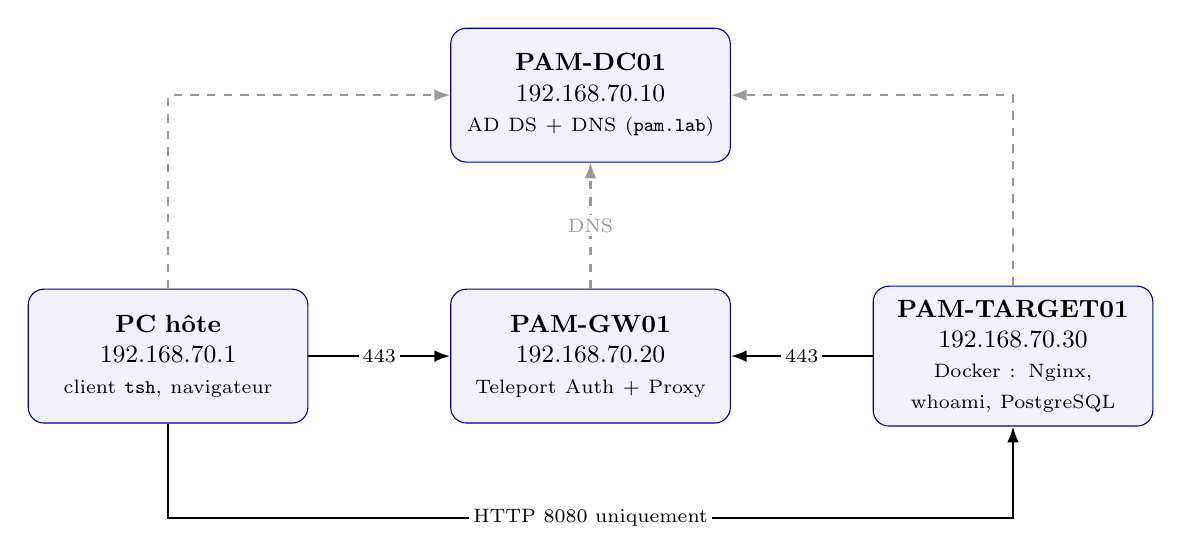
\begin{tikzpicture}[
  font=\small,
  box/.style={draw=blue!55!black,fill=blue!5,rounded corners=2mm,align=center,
    text width=3.2cm,minimum height=1.7cm,inner sep=5pt},
  flow/.style={-{Latex[length=2mm]},thick},
  dns/.style={-{Latex[length=2mm]},thick,dashed,gray!80},
  lab/.style={font=\scriptsize,fill=white,inner sep=1.5pt}
]
\node[box] (pc) {\textbf{PC hôte}\par 192.168.70.1\par\scriptsize client \texttt{tsh}, navigateur};
\node[box,right=18mm of pc] (gw) {\textbf{PAM-GW01}\par 192.168.70.20\par\scriptsize Teleport Auth + Proxy};
\node[box,right=18mm of gw] (tg) {\textbf{PAM-TARGET01}\par 192.168.70.30\par\scriptsize Docker : Nginx, whoami, PostgreSQL};
\node[box,above=16mm of gw] (dc) {\textbf{PAM-DC01}\par 192.168.70.10\par\scriptsize AD DS + DNS (\texttt{pam.lab})};

\draw[flow] (pc) -- (gw) node[lab,midway] {443};
\draw[flow] (tg) -- (gw) node[lab,midway] {443};
\draw[flow] (pc.south) -- ++(0,-12mm) -| (tg.south) node[lab,pos=0.25] {HTTP 8080 uniquement};
\draw[dns] (pc.north) |- (dc.west);
\draw[dns] (gw.north) -- (dc.south) node[lab,midway] {DNS};
\draw[dns] (tg.north) |- (dc.east);
\end{tikzpicture}
\caption{Architecture réalisée. Flèches pleines : flux autorisés et testés ; pointillés : résolution DNS. L'agent de TARGET01 ouvre lui-même le tunnel \emph{sortant} vers le Proxy ; aucun port SSH entrant n'est nécessaire sur la cible.}
\label{fig:archi-reelle}
\end{figure}

Deux autorités de certification coexistent : une autorité de laboratoire créée avec \texttt{openssl} pour le certificat TLS du Proxy (\texttt{pam-gw01.pam.lab}, SAN DNS et IP), et l'autorité interne de Teleport pour les certificats d'utilisateurs et d'hôtes. Le certificat du Proxy est reconnu sans option \texttt{-k} une fois l'autorité de laboratoire ajoutée aux magasins de confiance.

\section{Active Directory et DNS}
Le contrôleur de domaine PAM-DC01 héberge le domaine \texttt{pam.lab} (niveau fonctionnel Windows 2016). L'inspection en lecture seule a confirmé le rôle de contrôleur de domaine (\texttt{DomainRole} 5), les services NTDS, DNS, Kdc et W32Time en fonctionnement et le service DHCP désactivé. Un enregistrement DNS A \texttt{pam-gw01.pam.lab $\rightarrow$ 192.168.70.20} a été ajouté.

\textbf{Rôle exact d'AD dans cette réalisation.} Active Directory fournit le domaine et la résolution de noms. Les machines Linux ne sont \emph{pas} jointes au domaine et les utilisateurs Teleport sont des comptes locaux : Teleport Community Edition ne propose comme SSO externe que GitHub, l'authentification OIDC, SAML ou Active Directory relevant des éditions Enterprise (documentation consultée le 14 octobre 2026 ; URL exacte de la matrice des fonctions à ajouter à la bibliographie \aconf). Toute correspondance entre groupes AD et rôles Teleport serait manuelle et ne constituerait pas une intégration.

\textbf{Dépendance constatée.} L'agent de TARGET01 se connecte au Proxy par son nom. Après un démarrage à froid, \texttt{pam-target01} est resté absent de \texttt{tctl nodes ls} tant que DC-01 (DNS) n'était pas démarré, puis s'est reconnecté. Le DNS d'AD est donc une dépendance réelle du chemin PAM.

\section{Déploiement de Teleport}
\textbf{Licence.} Depuis la version~16, l'édition Community est gratuite pour les particuliers et les entreprises de moins de 100 salariés et de moins de 10~M\$ de chiffre d'affaires~\cite{tp-licence} ; un laboratoire étudiant entre dans ce cadre (lecture de l'équipe, non avis juridique). Les demandes d'accès à la demande (\emph{just-in-time}) ne sont disponibles qu'en ligne de commande dans cette édition.

\textbf{Installation sur PAM-GW01.}
\begin{enumerate}
\item Installation de Teleport 18.11.3 depuis le dépôt apt officiel au moyen du script du fournisseur (somme SHA-256 du script vérifiée).
\item Création de l'autorité de laboratoire et du certificat serveur ; \texttt{openssl verify} affiche \texttt{OK}.
\item \texttt{teleport configure} avec ce certificat, démarrage du service, réponse HTTPS sans \texttt{-k} ; authentification locale avec second facteur \texttt{otp}.
\end{enumerate}

\textbf{Enrôlement de PAM-TARGET01.} Le nœud est enregistré sous le nom \texttt{pam-target01} avec les étiquettes \texttt{env=lab} et \texttt{role=docker-host}, au moyen d'un jeton valable 15~minutes. La connexion est un tunnel inverse sortant de la cible vers le Proxy.

\textbf{Client.} \texttt{tsh} 18.11.3 a été installé sur le PC ; la somme SHA-256 de l'archive correspond à la valeur publiée par l'éditeur.

\section{Services Docker sur PAM-TARGET01}
Trois conteneurs sont décrits par un projet Compose : Nginx, \texttt{traefik/whoami} (application de test) et \texttt{postgres:16}. Nginx est publié sur \texttt{192.168.70.30:8080} uniquement ; PostgreSQL n'est pas publié, et le réseau Compose \texttt{internal} sépare les composants. L'utilisateur d'administration n'a pas été ajouté au groupe \texttt{docker}.

Observations : les trois services sont \texttt{Up} ; \texttt{curl http://192.168.70.30:8080} renvoie la réponse de \texttt{whoami} à travers Nginx ; \texttt{ss -tlnp} ne montre que le port 8080 (processus \texttt{docker-proxy}) et aucun écouteur sur 5432. Le conteneur applicatif \texttt{whoami} n'interroge pas PostgreSQL : l'accessibilité de la base est donc testée au niveau réseau et avec \texttt{psql} dans le conteneur, et non par une requête applicative.

\section{Rôles et utilisateurs implémentés}\label{sec:roles-impl}
Quatre rôles Teleport ont été créés, avec un utilisateur par rôle, tous protégés par un mot de passe et un second facteur TOTP. Sur PAM-TARGET01, deux comptes Linux ont été créés : \texttt{sysadmin} (sudo sans mot de passe, connexion par mot de passe impossible) et \texttt{appop} (aucun sudo, hors du groupe \texttt{docker}). Teleport ne crée pas d'autorisation Linux : il limite \emph{quel compte Linux} chaque rôle peut utiliser, et ce sont les permissions Linux qui produisent les refus \texttt{sudo} et \texttt{docker}.

\footnotesize\setlength{\tabcolsep}{3pt}
\begin{longtable}{@{}p{1.9cm}p{1.5cm}p{1.5cm}p{1.2cm}p{4.2cm}p{4.6cm}@{}}
\caption{Rôles implémentés : ce que chacun peut et ne peut pas faire (résultats observés)}\\
\toprule\textbf{Rôle} & \textbf{Utilisateur} & \textbf{Compte Linux} & \textbf{Validité} & \textbf{Peut} & \textbf{Ne peut pas}\\ \midrule\endhead
\texttt{infra-admin} (profil AI) & \texttt{u-infra} & \texttt{sysadmin} & 8~h & Ouvrir une session SSH via Teleport sur \texttt{pam-target01} ; exécuter des commandes avec \texttt{sudo} sans mot de passe, dont \texttt{docker ps} & Administrer Teleport ; se connecter hors du chemin Teleport\\
\texttt{app-operator} (profil OA) & \texttt{u-appop} & \texttt{appop} & 2~h & Ouvrir une session SSH comme \texttt{appop} ; exécuter des commandes non privilégiées (\texttt{whoami}) & Utiliser \texttt{sudo} (refusé) ; utiliser \texttt{docker} (refusé) ; se connecter comme \texttt{sysadmin} (refusé par Teleport)\\
\texttt{limited-user} (profil UL) & \texttt{u-limited} & aucun & 2~h & S'authentifier (mot de passe + OTP) & Ouvrir une session SSH sur toute ressource, quel que soit le compte (refusé par Teleport)\\
\texttt{pam-admin} (profil AP) & \texttt{pam-admin} & aucun & --- & Administrer Teleport (rôles \texttt{editor} et \texttt{auditor}), consulter le journal d'audit et les enregistrements & Ouvrir une session SSH : aucune ressource ne lui est visible\\
\bottomrule
\end{longtable}
\normalsize
Le profil analyste sécurité (AS) de la matrice du chapitre~4 n'est pas encore implémenté : il dépend de Wazuh. En attendant, le rôle \texttt{auditor} de \texttt{pam-admin} permet de lire l'audit Teleport. Les rôles portent la contrainte d'étiquette \texttt{env: lab}, ce qui limite leur portée aux ressources du laboratoire. Le compte \texttt{sysadmin} dispose de privilèges root permanents sur la cible : le contrôle repose ici sur l'attribution du rôle, la durée de vie du certificat et l'audit (voir limites).

\section{Tests d'autorisation observés}
\footnotesize\setlength{\tabcolsep}{3pt}
\begin{longtable}{@{}p{0.8cm}p{3.9cm}p{2.4cm}p{5.3cm}p{1.8cm}@{}}
\caption{Résultats observés des tests d'autorisation (14 octobre 2026)}\\
\toprule\textbf{N\textdegree} & \textbf{Acteur et action} & \textbf{Attendu} & \textbf{Observé} & \textbf{Résultat}\\ \midrule\endhead
A1 & \texttt{u-infra} se connecte (mot de passe + OTP) & Succès, rôle \texttt{infra-admin} & \texttt{Logged in as u-infra}, \texttt{Roles: infra-admin}, \texttt{Logins: sysadmin}, valide 7~h~59 & Réussi\\
A2 & \texttt{u-infra} : \texttt{tsh ssh sysadmin@pam-target01} avec \texttt{whoami; hostname; sudo -n docker ps} & Autorisé & \texttt{sysadmin}, \texttt{pam-target01}, trois conteneurs listés & Réussi (T02)\\
A3 & \texttt{u-appop} se connecte & Succès, rôle \texttt{app-operator} & Connexion réussie, valide 1~h~59 & Réussi\\
A4 & \texttt{u-appop} : \texttt{whoami} sur la cible & Autorisé & \texttt{appop} & Réussi\\
A5 & \texttt{u-appop} : \texttt{sudo -n true} & Refusé & \texttt{sudo: a password is required} & Réussi (T03)\\
A6 & \texttt{u-appop} : \texttt{docker ps} & Refusé & \texttt{permission denied} sur \texttt{docker.sock} & Réussi (T05)\\
A7 & \texttt{u-appop} : \texttt{tsh ssh sysadmin@pam-target01} & Refusé par Teleport & \texttt{access denied to sysadmin connecting to pam-target01} & Réussi\\
A8 & \texttt{u-limited} se connecte puis \texttt{tsh ssh appop@pam-target01} & Connexion réussie, SSH refusé & Connexion réussie, liste de comptes vide ; \texttt{access denied to appop connecting to pam-target01} & Réussi\\
\bottomrule
\end{longtable}
\normalsize
Les huit vérifications ont donné le résultat attendu. Il s'agit d'un sous-ensemble provisoire : l'indicateur d'exactitude RBAC du chapitre~4 sera calculé sur la matrice finale de tests, et non sur ces huit lignes. Les refus A5 et A6 proviennent des permissions Linux ; l'apport de Teleport est de restreindre le compte utilisable (A7, A8).

\section{Preuves d'audit}
Le journal d'audit de Teleport (heures UTC) contient, entre autres :
\begin{itemize}
\item 10:57:46 \texttt{Local Login Failed [missing second factor]} pour \texttt{u-infra} (code OTP omis par erreur) : un échec d'authentification est bien journalisé ;
\item 10:59:52, 11:00:03 et 11:00:05 : début de session, exécution de commande et fin de session de \texttt{u-infra} sur \texttt{pam-target01} ;
\item 11:01:28 \texttt{Command Execution Failed [exit status 1]} pour \texttt{u-appop} (tentative \texttt{sudo}/\texttt{docker}) ;
\item 11:02:02 \texttt{Auth Attempt Failed} : \texttt{u-appop}, compte « sysadmin » absent des comptes valides \texttt{["appop"]} ;
\item 11:02:59 \texttt{Auth Attempt Failed} : \texttt{u-limited}, compte « appop » absent des comptes valides ;
\item 11:04:21 à 11:04:51 : session interactive de \texttt{u-infra} (17~s), avec événement \texttt{Session Uploaded}.
\end{itemize}
L'enregistrement de session d'identifiant \texttt{bab664dd-5180-4704-bee2-705bad45eec8} apparaît à la fois dans l'audit et dans l'enregistrement, où les commandes \texttt{whoami} et \texttt{sudo docker ps} sont visibles. Les événements de mise en place (création d'utilisateurs, jetons, ajout d'appareils MFA, émission de certificats) sont également journalisés. L'heure de l'enregistrement (12:04 locale) correspond à l'heure d'audit (11:04 UTC) : GW01 et le PC sont cohérents.

\section{Pare-feu : règles appliquées et tests}
Les règles ont été appliquées le 16 octobre 2026, avec une minuterie de retour arrière de 15~minutes (\texttt{systemd-run}) comme filet de sécurité, annulée après validation. Elles mettent en œuvre l'option~B du chapitre~4 (pare-feu natifs, sans machine supplémentaire).

\subsection{Règles}
\textbf{PAM-TARGET01.} \texttt{ufw} actif, politique « refuser » en entrée et « autoriser » en sortie, \emph{aucune} règle d'autorisation SSH. Comme les ports publiés par Docker contournent les règles \texttt{INPUT} d'\texttt{ufw}~\cite{docker-fw}, la chaîne \texttt{DOCKER-USER} contient : (1) \texttt{RETURN} pour TCP depuis 192.168.70.1 vers le port 8080 sur \texttt{ens33} ; (2) \texttt{DROP} pour le reste du trafic entrant sur \texttt{ens33} ; (3) \texttt{RETURN}. Ces règles sont reconstruites au démarrage par le service \texttt{docker-user-fw.service} (installé et activé).

\textbf{PAM-GW01.} \texttt{ufw} avec politique « refuser » en entrée ; autorisation de 443/tcp depuis 192.168.70.1 (PC) et 192.168.70.30 (TARGET01) ; autorisation de 22/tcp depuis 192.168.70.1 seulement.

\subsection{Résultats}
\footnotesize\setlength{\tabcolsep}{3pt}
\begin{longtable}{@{}p{0.8cm}p{5.0cm}p{2.2cm}p{3.3cm}p{3.2cm}@{}}
\caption{Tests de filtrage avant/après (16 octobre 2026)}\\
\toprule\textbf{N\textdegree} & \textbf{Test} & \textbf{Avant} & \textbf{Après} & \textbf{Résultat}\\ \midrule\endhead
F1 & GW01 $\rightarrow$ TARGET01:22 (connexion TCP) & ouvert & fermé/filtré & Réussi\\
F2 & GW01 $\rightarrow$ TARGET01:8080 & ouvert & fermé/filtré & Réussi\\
F3 & GW01 $\rightarrow$ TARGET01:5432 & fermé/filtré & fermé/filtré & Réussi (port jamais publié)\\
F4 & PC $\rightarrow$ \texttt{http://192.168.70.30:8080} & réponse & réponse & Réussi (source autorisée)\\
F5 & PC $\rightarrow$ nouvelle connexion SSH vers 192.168.70.30:22 & non exécuté & \texttt{Connection timed out} & Réussi\\
F6 & PC $\rightarrow$ \texttt{tsh ssh sysadmin@pam-target01 whoami}, SSH direct bloqué & fonctionne & \texttt{sysadmin} & Réussi (chemin PAM intact)\\
F7 & TARGET01 $\rightarrow$ GW01:443 et :22 après pare-feu de GW01 & non exécuté & 443 ouvert, 22 fermé/filtré & Réussi\\
F8 & Redémarrage de l'agent de TARGET01 puis \texttt{tctl nodes ls} & non exécuté & \texttt{pam-target01} listé & Réussi\\
F9 & PC $\rightarrow$ \texttt{tsh ssh} à travers le pare-feu de GW01 (nouvelle session sur 443) & non exécuté & \texttt{sysadmin} & Réussi\\
\bottomrule
\end{longtable}
\normalsize

Ces résultats illustrent la complémentarité décrite au chapitre~4 : le SSH direct vers la cible est refusé aux nouvelles connexions (F5) alors que l'accès par le PAM fonctionne toujours (F6, F9), parce que le tunnel est initié par la cible vers le Proxy et que la règle de GW01 autorise ce flux entrant sur 443 (F7, F8). Les tests F1 à F9 correspondent à une exécution \textbf{partielle} des tests T13, T14 et T15 : ils ont été menés depuis GW01 et le PC, non depuis Kali.

\subsection{Observations à signaler}
\begin{itemize}
\item Une session SSH du PC déjà ouverte avant l'application des règles est restée active : le pare-feu est à états, les règles ne s'appliquent qu'aux nouvelles connexions.
\item Une première mesure « avant » était invalide (TARGET01 éteinte) et a été refaite ; seules les valeurs valides figurent dans le tableau.
\item GW01 accepte toujours le SSH depuis le PC : c'est un chemin d'administration hors Teleport, conservé pour la mise au point et à supprimer avant les tests finaux s'il n'est plus nécessaire.
\item Le DNS vers DC-01 doit rester autorisé (dépendance de l'agent, section précédente).
\end{itemize}

\section{Difficultés rencontrées et corrections}
\begin{itemize}
\item L'adaptateur VMnet1 de l'hôte avait une adresse 169.254.x.x : adresse statique 192.168.70.1/24 configurée. Les premiers pings ont échoué tant que l'adresse était à l'état provisoire ; le ping de GW01 vers l'hôte a nécessité une règle entrante ICMP limitée au sous-réseau du laboratoire et à l'adaptateur VMnet1.
\item L'adaptateur NAT de GW01 a exigé son propre fichier netplan (\texttt{ens37}).
\item \texttt{teleport configure} a d'abord échoué car les fichiers de certificat étaient dans le dossier personnel et non dans \texttt{/var/lib/teleport} ; le service redémarrait en boucle jusqu'au déplacement des fichiers et à la régénération de la configuration.
\item Un délai de résolution DNS de \texttt{pam-gw01.pam.lab} a été observé sur TARGET01 au démarrage, résolu au nouvel essai (connexion de l'agent 13~s plus tard).
\item La création des utilisateurs Linux a d'abord été lancée sur GW01 par erreur ; elle a été annulée sur GW01 puis refaite sur TARGET01.
\item Un code OTP a été soumis vide (\texttt{missing second factor}) ; la connexion a réussi à l'essai suivant.
\end{itemize}

\section{Limites et compromis assumés}
\begin{itemize}
\item AD ne fournit que le DNS et le domaine ; les VM Linux ne sont pas jointes au domaine et les utilisateurs Teleport sont locaux (limite de l'édition Community).
\item GW01 (Teleport) et TARGET01 (ressource protégée) sont deux VM distinctes, conformément à la recommandation du chapitre~4 ; la clé privée de l'autorité de laboratoire réside sur GW01 par commodité.
\item \texttt{sysadmin} dispose de privilèges root permanents ; la maîtrise repose sur le rôle, la durée du certificat et l'audit.
\item L'application \texttt{whoami} ne sollicite pas PostgreSQL.
\item Les paquets Docker proviennent des dépôts Ubuntu, plus anciens que ceux de Docker.
\item L'autorité de laboratoire est installée dans le magasin utilisateur du PC ; elle sera retirée à la fin du projet.
\item GW01 et TARGET01 possèdent encore un adaptateur NAT temporaire (accès Internet) à supprimer ou bloquer avant les tests de pare-feu finaux.
\end{itemize}

\section{Travaux restants}\label{sec:reste}
Les éléments suivants n'ont \textbf{pas} été exécutés et ne sont pas présentés comme réussis.
\begin{itemize}
\item Persistance du pare-feu après redémarrage de TARGET01 ; Windows Defender Firewall sur DC-01 et sur le PC ; filtrage sortant ; journalisation du pare-feu (T17) ; régression complète (T18).
\item Machine Kali : disponibilité non confirmée ; scan de ports (T16) et tentatives de contournement non réalisés ; test PostgreSQL (T14) depuis une machine non autorisée non réalisé.
\item Wazuh : Docker Desktop n'était pas démarré lors de la vérification ; aucun agent installé, aucune remontée de journaux, donc ni détection (T07) ni corrélation (T10) ; profil AS non implémenté.
\item Révocation et expiration des accès (à vérifier d'abord dans la documentation Teleport).
\item Examen de certains détails d'audit (texte des commandes, adresse source, quatre événements \texttt{Certificate Issued} de \texttt{u-limited} à 11:00:27 UTC).
\item Synchronisation d'horloge de TARGET01 et de DC-01 non vérifiée.
\item Suppression des adaptateurs NAT temporaires ; calcul des indicateurs finaux (aucune valeur finale n'est établie à ce stade).
\end{itemize}

%================= BIBLIOGRAPHIE =================
\chapter*{Bibliographie et webographie}
\addcontentsline{toc}{chapter}{Bibliographie et webographie}
\small
\textit{Sources consultées le 12 octobre 2026. Celles marquées $\dagger$ sont à vérifier avant le rendu final (non ouvertes pendant la rédaction ou version de documentation à confirmer).}
\begin{thebibliography}{99}
\bibitem{tp-keycloak} Teleport, « Keycloak SSO », documentation (URL fournie dans le cahier des charges) : \url{https://goteleport.com/docs/zero-trust-access/sso/integrate-idp/keycloak/} $\dagger$.
\bibitem{tp-licence} Teleport, « Teleport Community Edition will adopt a commercial license starting with version 16 » : \url{https://goteleport.com/blog/teleport-community-license}.
\bibitem{tp-net} Teleport, « Networking Reference » : \url{https://goteleport.com/docs/reference/deployment/networking/}.
\bibitem{wazuh-arch} Wazuh, « Architecture » (documentation de la branche 5.0, candidate au moment de la consultation) : \url{https://documentation.wazuh.com/5.0-rc/getting-started/architecture.html} $\dagger$ ; version déployée à confirmer.
\bibitem{wazuh-enrol} Wazuh, « Agent enrollment requirements » : \url{https://documentation.wazuh.com/current/user-manual/agent/agent-enrollment/requirements.html}.
\bibitem{jumpserver} JumpServer, dépôt officiel : \url{https://github.com/jumpserver/jumpserver}.
\bibitem{swi} Start with Identity, « Top 7 Open-Source PAM Solutions » (source indépendante) : \url{https://startwithidentity.com/articles/top-7-open-source-pam-solutions/} $\dagger$.
\bibitem{docker-sec} Docker, « Docker Engine security » : \url{https://docs.docker.com/engine/security/}.
\bibitem{docker-fw} Docker, « Packet filtering and firewalls » : \url{https://docs.docker.com/network/packet-filtering-firewalls/}.
\bibitem{baeldung-ufw} Baeldung, « Docker published ports ignoring ufw rules » (source indépendante) : \url{https://www.baeldung.com/linux/docker-container-published-port-ignoring-ufw-rules}.
\bibitem{ubuntu-fw} Ubuntu, « Firewall » : \url{https://documentation.ubuntu.com/security/security-features/network/firewall/}.
\bibitem{ufw-wiki} Ubuntu Wiki, « UncomplicatedFirewall » : \url{https://wiki.ubuntu.com/UncomplicatedFirewall}.
\bibitem{vmware-ho} Broadcom, « Understanding networking types in hosted products » : \url{https://knowledge.broadcom.com/external/article/309842/understanding-networking-types-in-hosted.html}.
\bibitem{vmware-ho-doc} VMware, « Configuring Host-Only Networking » (Workstation Pro 17) : \url{https://docs.vmware.com/en/VMware-Workstation-Pro/17/com.vmware.ws.using.doc/GUID-93BDF7F1-D2E4-42CE-80EA-4E305337D2FC.html} $\dagger$.
\bibitem{vmware-multi} VMware, « Add a Host-Only Virtual Network » (Workstation Pro 17) : \url{https://docs.vmware.com/en/VMware-Workstation-Pro/17/com.vmware.ws.using.doc/GUID-E08995A9-7DE6-4D92-8C6F-4F737C3A8AB3.html} $\dagger$.
\end{thebibliography}
\textit{Vérifications bibliographiques avant remise : confirmer les pages et versions effectivement consultées, en particulier les pages Teleport, Wazuh et VMware marquées d'un symbole dans les brouillons antérieurs. Ajouter la documentation Microsoft officielle sur les ports AD DS/DNS et Windows Defender Firewall, ainsi que la documentation Keycloak et la référence NIST SP~800-92 si ces éléments sont effectivement utilisés. Ne conserver dans la bibliographie finale que les sources consultées et citées dans le texte.}
\normalsize

%================= DECISIONS =================

\end{document}